\documentclass[times,astrosymb]{aastex631}
\usepackage{xspace}
\usepackage[utf8]{inputenc}


\newcommand{\paa}{Pa\ensuremath{\alpha}}
\newcommand{\brg}{Br\ensuremath{\gamma}}
\newcommand{\msun}{\ensuremath{M_{\odot}}\xspace}			%  Msun
\newcommand{\mdot}{\ensuremath{\dot{M}}\xspace}
\newcommand{\lsun}{\ensuremath{L_{\odot}}\xspace}			%  Lsun
\newcommand{\rsun}{\ensuremath{R_{\odot}}\xspace}			%  Rsun
\newcommand{\lbol}{\ensuremath{L_{\mathrm{bol}}\xspace}}	%  Lbol
\newcommand{\ks}{K\ensuremath{_{\mathrm{s}}}}		%  Ks
\newcommand{\hh}{\ensuremath{\textrm{H}_{2}}\xspace}			%  H2
\newcommand{\dens}{\ensuremath{n(\hh) [\percc]}\xspace}
\newcommand{\formaldehyde}{\ensuremath{\textrm{H}_2\textrm{CO}}\xspace}
\newcommand{\formamide}{\ensuremath{\textrm{NH}_2\textrm{CHO}}\xspace}
\newcommand{\formaldehydeIso}{\ensuremath{\textrm{H}_2~^{13}\textrm{CO}}\xspace}
\newcommand{\methanol}{\ensuremath{\textrm{CH}_3\textrm{OH}}\xspace}
\newcommand{\methane}{\ensuremath{\textrm{CH}_4}\xspace}
\newcommand{\ortho}{\ensuremath{\textrm{o-H}_2\textrm{CO}}\xspace}
\newcommand{\para}{\ensuremath{\textrm{p-H}_2\textrm{CO}}\xspace}
\newcommand{\oneone}{\ensuremath{1_{1,0}-1_{1,1}}\xspace}
\newcommand{\twotwo}{\ensuremath{2_{1,1}-2_{1,2}}\xspace}
\newcommand{\threethree}{\ensuremath{3_{1,2}-3_{1,3}}\xspace}
\newcommand{\threeohthree}{\ensuremath{3_{0,3}-2_{0,2}}\xspace}
\newcommand{\threetwotwo}{\ensuremath{3_{2,2}-2_{2,1}}\xspace}
\newcommand{\threetwoone}{\ensuremath{3_{2,1}-2_{2,0}}\xspace}
\newcommand{\fourtwotwo}{\ensuremath{4_{2,2}-3_{1,2}}\xspace} % CH3OH 218.4 GHz
\newcommand{\methylcyanide}{\ensuremath{\textrm{CH}_{3}\textrm{CN}}\xspace}
\newcommand{\ketene}{\ensuremath{\textrm{H}_{2}\textrm{CCO}}\xspace}
\newcommand{\ethylcyanide}{\ensuremath{\textrm{CH}_3\textrm{CH}_2\textrm{CN}}\xspace}
\newcommand{\cyanoacetylene}{\ensuremath{\textrm{HC}_{3}\textrm{N}}\xspace}
\newcommand{\methylformate}{\ensuremath{\textrm{CH}_{3}\textrm{OCHO}}\xspace}
\newcommand{\dimethylether}{\ensuremath{\textrm{CH}_{3}\textrm{OCH}_{3}}\xspace}
\newcommand{\gaucheethanol}{\ensuremath{\textrm{g-CH}_3\textrm{CH}_2\textrm{OH}}\xspace}
\newcommand{\acetone}{\ensuremath{\left[\textrm{CH}_{3}\right]_2\textrm{CO}}\xspace}
\newcommand{\methyleneamidogen}{\ensuremath{\textrm{H}_{2}\textrm{CN}}\xspace}
\newcommand{\Rone}{\ensuremath{\para~S_{\nu}(\threetwoone) / S_{\nu}(\threeohthree)}\xspace}
\newcommand{\Rtwo}{\ensuremath{\para~S_{\nu}(\threetwotwo) / S_{\nu}(\threetwoone)}\xspace}
\newcommand{\JKaKc}{\ensuremath{J_{K_a K_c}}}
\newcommand{\water}{H$_{2}$O\xspace}		%  H2O
\newcommand{\feii}{\ion{Fe}{ii}\xspace}		%  FeII

\newcommand{\uchii}{\ion{UCH}{ii}\xspace}
\newcommand{\UCHII}{\ion{UCH}{ii}\xspace}
\newcommand{\hchii}{\ion{HCH}{ii}\xspace}
\newcommand{\HCHII}{\ion{HCH}{ii}\xspace}
\newcommand{\hii}{\ion{H}{ii}\xspace}

\newcommand{\hi}{H~{\sc i}\xspace}
\newcommand{\Hii}{\hii}
\newcommand{\HII}{\hii}
\newcommand{\Xform}{\ensuremath{X_{\formaldehyde}}}
\newcommand{\kms}{\textrm{km~s}\ensuremath{^{-1}}\xspace}	%  km s-1
\newcommand{\nsample}{456\xspace}
\newcommand{\CFR}{5\xspace} % nMPC / 0.25 / 2 (6 for W51 once, 8 for W51 twice) REFEDIT: With f_observed=0.3, becomes 3/2./0.3 = 5
\newcommand{\permyr}{\ensuremath{\mathrm{Myr}^{-1}}\xspace}
\newcommand{\pers}{\ensuremath{\mathrm{s}^{-1}}\xspace}
\newcommand{\perspc}{\ensuremath{\mathrm{pc}^{-2}}\xspace}
\newcommand{\tsuplim}{0.5\xspace} % upper limit on starless timescale
\newcommand{\ncandidates}{18\xspace}
\newcommand{\mindist}{8.7\xspace}
\newcommand{\rcluster}{2.5\xspace}
\newcommand{\ncomplete}{13\xspace}
\newcommand{\middistcut}{13.0\xspace}
\newcommand{\nMPC}{3\xspace} % only count W51 once.  W51, W49, G010
\newcommand{\obsfrac}{30}
\newcommand{\nMPCtot}{10\xspace} % = nmpc / obsfrac
\newcommand{\nMPCtoterr}{6\xspace} % = sqrt(nmpc) / obsfrac
\newcommand{\plaw}{2.1\xspace}
\newcommand{\plawerr}{0.3\xspace}
\newcommand{\mmin}{\ensuremath{10^4~\msun}\xspace}
%\newcommand{\perkmspc}{\textrm{per~km~s}\ensuremath{^{-1}}\textrm{pc}\ensuremath{^{-1}}\xspace}	%  km s-1 pc-1
\newcommand{\kmspc}{\textrm{km~s}\ensuremath{^{-1}}\textrm{pc}\ensuremath{^{-1}}\xspace}	%  km s-1 pc-1
\newcommand{\sqcm}{cm$^{2}$\xspace}		%  cm^2
\newcommand{\percc}{\ensuremath{\textrm{cm}^{-3}}\xspace}
\newcommand{\perpc}{\ensuremath{\textrm{pc}^{-1}}\xspace}
\newcommand{\persc}{\ensuremath{\textrm{cm}^{-2}}\xspace}
\newcommand{\persr}{\ensuremath{\textrm{sr}^{-1}}\xspace}
\newcommand{\peryr}{\ensuremath{\textrm{yr}^{-1}}\xspace}
\newcommand{\perkmspc}{\textrm{km~s}\ensuremath{^{-1}}\textrm{pc}\ensuremath{^{-1}}\xspace}	%  km s-1 pc-1
\newcommand{\perkms}{\textrm{per~km~s}\ensuremath{^{-1}}\xspace}	%  km s-1 
\newcommand{\um}{\ensuremath{\mu \textrm{m}}\xspace}    % micron
\newcommand{\microjy}{\ensuremath{\mu\textrm{Jy}}\xspace}    % micron
\newcommand{\microJy}{\ensuremath{\mu\textrm{Jy}}\xspace}    % micron
\newcommand{\mum}{\um}
\newcommand{\htwo}{\ensuremath{\textrm{H}_2}}
\newcommand{\Htwo}{\ensuremath{\textrm{H}_2}}
\newcommand{\HtwoO}{\ensuremath{\textrm{H}_2\textrm{O}}}
\newcommand{\htwoo}{\ensuremath{\textrm{H}_2\textrm{O}}}
\newcommand{\ha}{\ensuremath{\textrm{H}\alpha}}
\newcommand{\hb}{\ensuremath{\textrm{H}\beta}}
\newcommand{\so}{SO~\ensuremath{5_6-4_5}\xspace}
\newcommand{\SO}{SO~\ensuremath{1_2-1_1}\xspace}
\newcommand{\ammonia}{NH\ensuremath{_3}\xspace}
\newcommand{\twelveco}{\ensuremath{^{12}\textrm{CO}}\xspace}
\newcommand{\thirteenco}{\ensuremath{^{13}\textrm{CO}}\xspace}
\newcommand{\ceighteeno}{\ensuremath{\textrm{C}^{18}\textrm{O}}\xspace}
\def\ee#1{\ensuremath{\times10^{#1}}}
\newcommand{\degrees}{\ensuremath{^{\circ}}}
% can't have \degree because I'm getting a degree...
\newcommand{\lowirac}{800}
\newcommand{\highirac}{8000}
\newcommand{\lowmips}{600}
\newcommand{\highmips}{5000}
\newcommand{\perbeam}{\ensuremath{\textrm{beam}^{-1}}\xspace}
\newcommand{\ds}{\ensuremath{\textrm{d}s}}
\newcommand{\dnu}{\ensuremath{\textrm{d}\nu}}
\newcommand{\dv}{\ensuremath{\textrm{d}v}}
\def\secref#1{Section \ref{#1}}
\def\eqref#1{Equation \ref{#1}}
\def\facility#1{#1}
%\newcommand{\arcmin}{'}

\newcommand{\necluster}{Sh~2-233IR~NE}
\newcommand{\swcluster}{Sh~2-233IR~SW}
\newcommand{\region}{IRAS 05358}

\newcommand{\nwfive}{40}
\newcommand{\nouter}{15}

\newcommand{\vone}{{\rm v}1.0\xspace}
\newcommand{\vtwo}{{\rm v}2.0\xspace}
\newcommand\mjysr{\ensuremath{{\rm MJy~sr}^{-1}}}
\newcommand\jybm{\ensuremath{{\rm Jy~bm}^{-1}}}
\newcommand\nbolocat{8552\xspace}
\newcommand\nbolocatnew{548\xspace}
\newcommand\nbolocatnonew{8004\xspace} % = nbolocat-nbolocatnew
%\renewcommand\arcdeg{\mbox{$^\circ$}\xspace} 
%\renewcommand\arcmin{\mbox{$^\prime$}\xspace} 
%\renewcommand\arcsec{\mbox{$^{\prime\prime}$}\xspace} 

\newcommand{\todo}[1]{\textcolor{red}{#1}}
\newcommand{\okinfinal}[1]{{#1}}
%% only needed if not aastex
%\newcommand{\keywords}[1]{}
%\newcommand{\email}[1]{}
%\newcommand{\affil}[1]{}


%aastex hack
%\newcommand\arcdeg{\mbox{$^\circ$}}%
%\newcommand\arcmin{\mbox{$^\prime$}\xspace}%
%\newcommand\arcsec{\mbox{$^{\prime\prime}$}\xspace}%


% https://tex.stackexchange.com/a/687778/8546
\usepackage{tikz}
\usetikzlibrary{calc,tikzmark} 
\newlength{\imageheight}
%\settoheight{\imageheight}{% measure the image height
%    \includegraphics[width=4cm]{example-image} % your image <<<<<<<<<<<<<<<<<
%}

%\newcommand{\FontLabel}{\sffamily\bfseries\large}% set the font of the labels <<<<<<<<

%\newcommand{\InsertLabels}[2]{% 
%  \begin{tikzpicture}[overlay,remember picture]
%        \node[font=\FontLabel] at ( $ (pic cs:a) +(#1,\imageheight-#2) $ ){a};% 
%        \node[font=\FontLabel] at ( $ (pic cs:b) +(#1,\imageheight-#2) $ ){b};% 
%        \node[font=\FontLabel] at ( $ (pic cs:c) +(#1,\imageheight-#2) $ ){c};% 
%        \node[font=\FontLabel] at ( $ (pic cs:d) +(#1,\imageheight-#2) $ ){d};% 
%    \end{tikzpicture}   
%}
\def\todo#1{\textcolor{red}{#1}}

\begin{document}
\title{Brick 2221: Paper I - overview}
\author[0000-0001-6431-9633]{Adam Ginsburg}
\affiliation{Department of Astronomy, University of Florida, P.O. Box 112055, Gainesville, FL, USA}
% TODO: add other authors
\date{September 2022}
\subsection{Recombination line excess sources}
\label{sec:recomb}
\todo{This section is a work in progress.}
One of the key aims of 2221 is to identify accreting sources, expected to be primarily YSOs, by their recombination line excess emission \citep[e.g.,][]{Hartmann2016,Alcala2017}.

\todo{I intend to use these data but not sure how to verify them; right now it looks like 2/3 of the stars have ``excess" by this definition, which is wrong.
Update Dec 30: there are clear problems with the photometry; most or all of the huge-excess sources are not real stars at all and fail on many ``quality factor" criteria.
I'm still trying to determine if there are \emph{any} example sources that have legitimate excess.
Unfortunately it looks like a major concern here is astrometric matching between the frames, which I solved for the long-wavelength bands but not for the short-wavelength bands.
I'm trying again now though, using the astrometric solution for the long-wave bands as the reference for the short-wave bands.
}
We performed line- and continuum-subtraction in a manner similar to that for the star removal process (\S \ref{sec:starsub}).
We first produce line-free continuum measurements by subtracting $S_{410m405} = S_{410} - w_{405} S_{405}$, where $w_{405}=0.108$ is the ratio of the F405N/F410M filter widths.
We then create a continuum-subtracted line flux $S_{405m410} = S_{405}-S_{410m405}$.
In principle, we expect this to be negative - and therefore the magnitudes to be undefined - for stars with atmospheric absorption features.
We do the same for the Pa$\alpha$ F187N and F182M filters.

Simply using the F405N-F410N and F187N-F182M colors, we select stars with evidence for recombination line emission.
Stars with no emission will have zero color in these filter pairs, since they cover the same wavelengths.
Stars with excess absorption, i.e., very deep hydrogen line atmospheric absorption, will appear slightly red; since we have converted fluxes to the AB magnitude system using, A0 stars may appear red.
Blue colors in these filters indicates hydrogen recombination line excess.
While excess in either filter pair could be an indication of a photometric error (e.g., from overlap with a PSF artifact), excess in both filters is a firm indication of genuine excess.
However, there still remains some opportunity for error: while \texttt{crowdsource} is designed to separate stellar from background emission, the separation is imperfect, so sources laying on a strong extended nebular emission background may appear as excess sources.
There is a strong selection bias in our sample: all of the selected excess sources are intrinsically faint, which is partly enforced by requiring that sources are detected (but not saturated) in both bands \todo{I don't think I actually imposed that selection criterion, but it seems to still be present in the data?}.
With these caveats in mind, though, we find $>1000$ sources with $\Delta m < -2$, or $F_{narrow} > 6 F_{medium}$, or about 2\% of the sources detected in these four filters.

Figure \ref{fig:braexcessstars_on_cmd} shows the location of the H-line excess sources on our extended emission map for the NRCA module.
There is a dense cluster of sources in the HII region G000.208-0.003, which are likely to be misidentified as excess sources.
The remainder of the sources are widely distributed across the full field, with many laying directly along the line of sight to the darkest extinction region in The Brick.
Given the requirement for F187N detection, these sources are \emph{not} deeply embedded in The Brick, but are either on its near end or are in the foreground.
\todo{Why do these selection criteria avoid the regions outside the brick?
The first-order reason is that the F187/F182 sources are missing, but why?
There is \emph{less} extinction.
Maybe it's crowding?
}

We are not yet able to identify which of these sources are young stars and which are other emission line sources (e.g., cataclysmic variables).

\todo{The ratio of the Pa$\alpha$ / Br$\alpha$ line should be 4.23 \citep[][Table 14.2]{Draine2011} [TODOx2: check that this is true in Jy units?], which translates to $\Delta m = -2.5 \log 4.23 = 1.56$.
We observe a broad scatter around this value, with many bright sources exhibiting higher ratios - which is not allowed under case B recombination (I checked by looking at the Storey \& Hummer 1995 tables -  the ratio never deviates much from 3).
A quick search on ADS shows that CVs are generally modeled as Case B recombination, so I don't think a difference in the recombination line emission makes sense.
I'm still not confident enough in the data to say definitively that something is here;
I need to see which stars are showing the excess.  Maybe they're all just bad stars.
}

%To search for these excess sources, we plot the Br$\alpha$ vs Br$\alpha$ continuum (405m410-410m405 vs 405m410) color-magnitude diagram (Figure \ref{fig:bracmds}.
%However, this results in $\sim2/3$ of the stars apparently having Br$\alpha$ excess, which seems extremely unlikely and raises questions about the photometry.

\begin{figure}
    \centering
    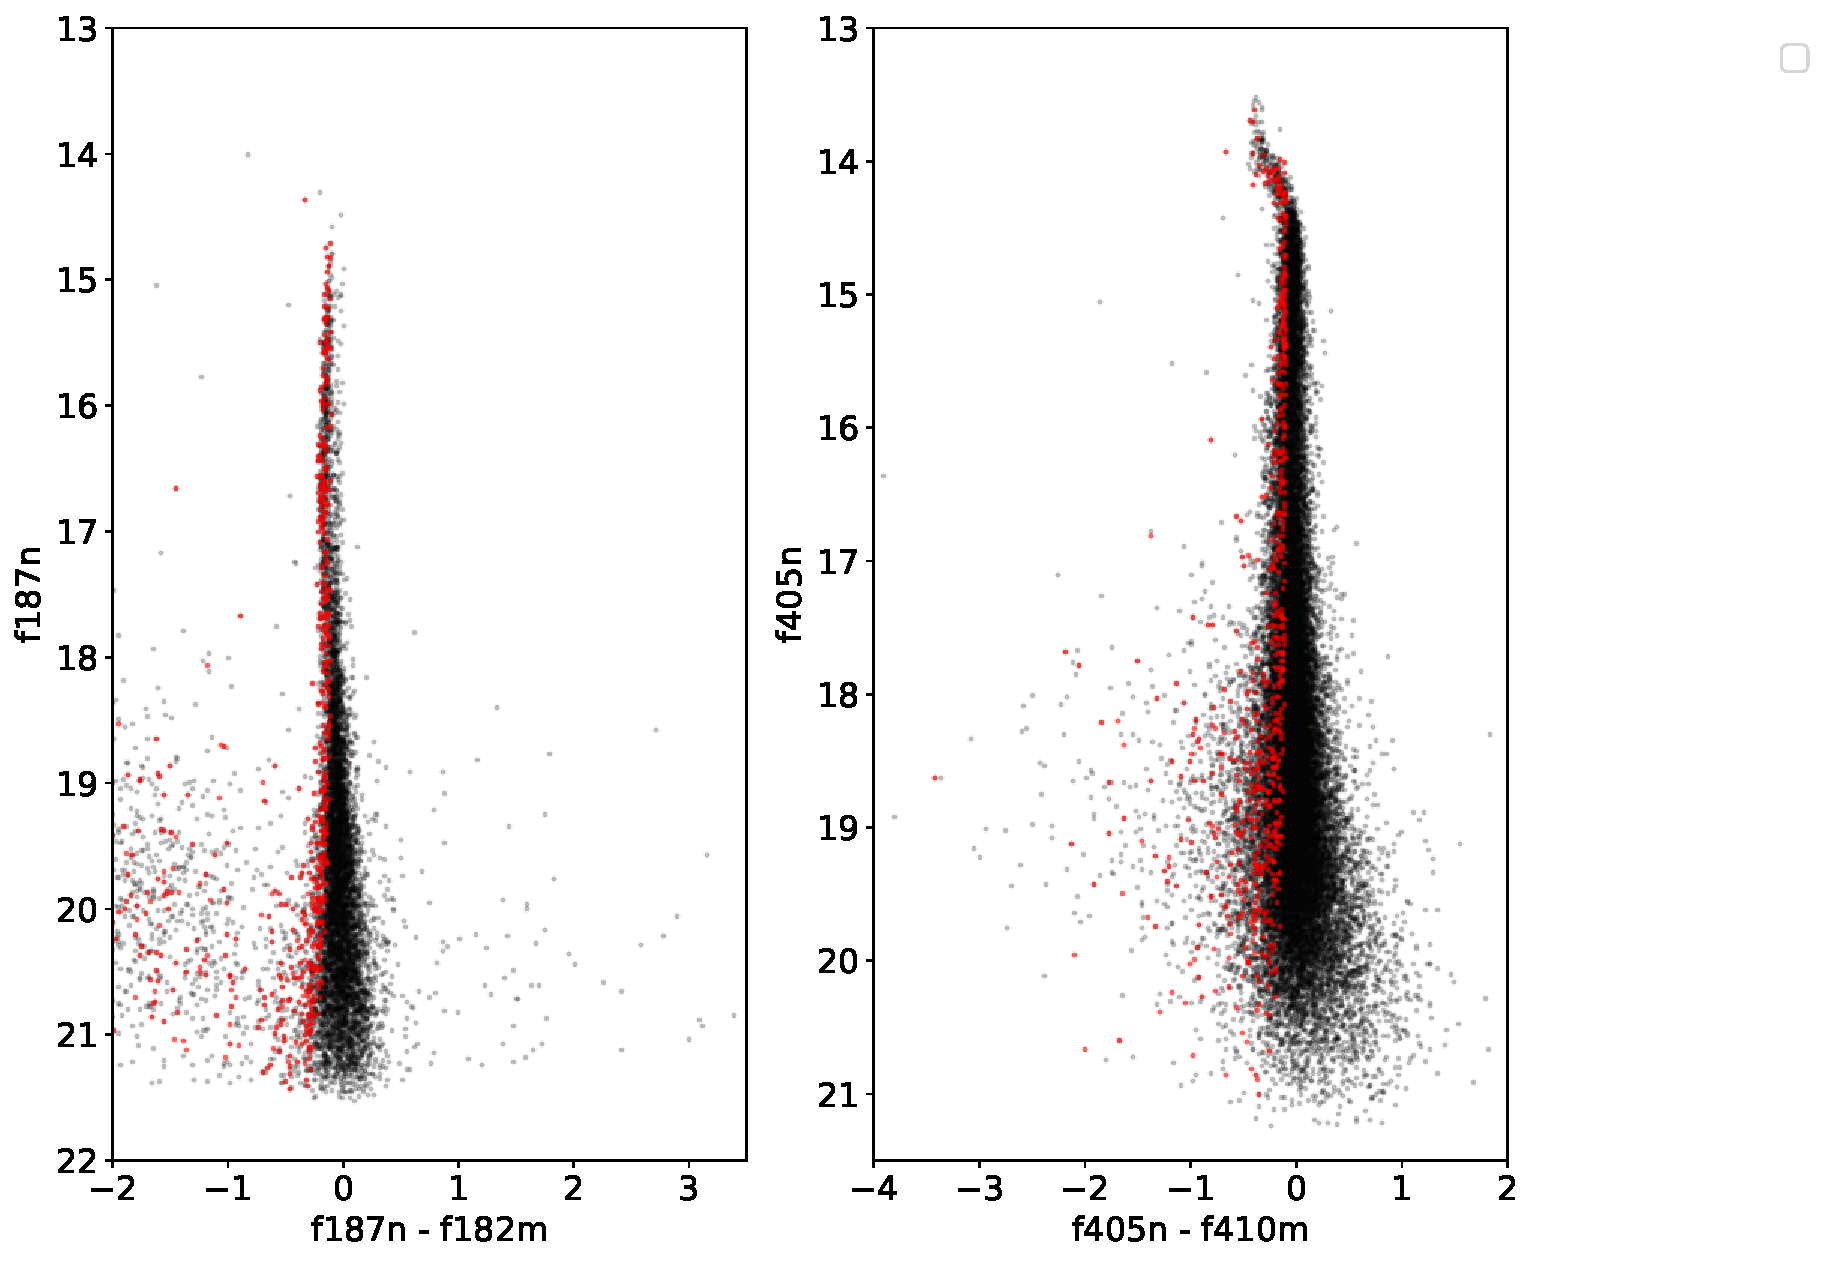
\includegraphics[width=\textwidth]{figures/BrA_PaA_CMDs.pdf}
    \caption{Brackett $\alpha$ (F405N) vs F410M color-magnitude diagrams.
    (left) The F187N-F182M CMD.
    %(left) The 410m405 vs 405m410 CMD.
    %Each point is a flux measurement in which the line (410m405) or continuum (405m410) has been subtracted (see \S \ref{sec:recomb}).
    (right) The F410M-F405N CMD.
    %These data points are the raw photometric data, with no attempt to subtract line or continuum from either filter.
    The red points are those where the recombination line filter is -0.1 magnitudes brighter than the broad-band filter in \emph{both} Pa$\alpha$ and Br$\alpha$.
    }
    \label{fig:bracmds}
\end{figure}

\begin{figure}
    \centering
    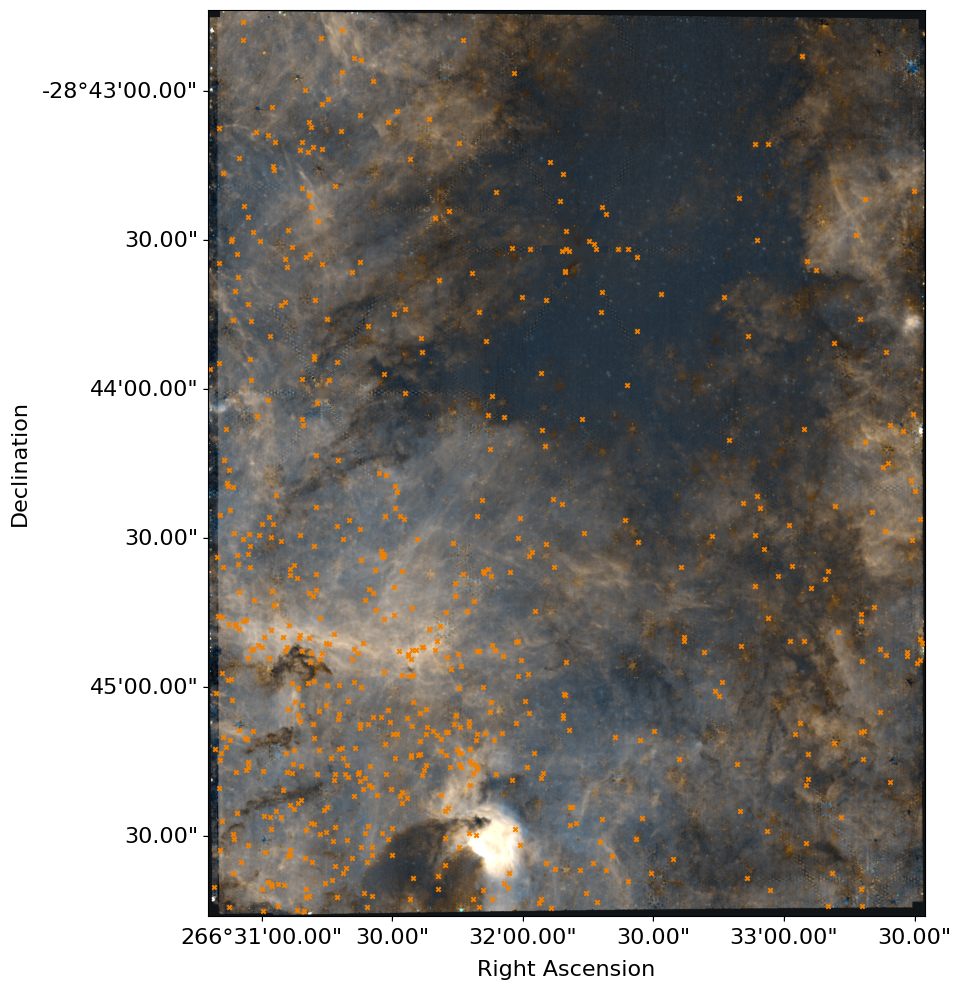
\includegraphics[width=\textwidth]{figures/BrAExcessStars_on_RGB.png}
    \caption{The Br$\alpha$ and Pa$\alpha$ excess stars from Figure \ref{fig:bracmds} overplotted on the star-removed three-color image from just the NRCA module (Fig \ref{fig:fullfieldstarless}.
    }
    \label{fig:braexcessstars_on_cmd}
\end{figure}

 \textit{Acknowledgements}
 We thank Eddie Schlafly and Andrew Saydjari for their assistance with \texttt{crowdsource} technical issues.
 AG acknowledges support from STSCI grant JWST-GO-02221.001-A, and from the NSF through AST 2008101, AST 220651, and CAREER 2142300.
 
\bibliography{bibliography}
\end{document}


% \subsection{Extinction}
% \todo{This section isn't doing anything right now}
% Based on both MIST and Padova isochrones \citep{}, stars have effectively zero color over all ages over most of our filters.
% However, at the youngest ages ($t<10^5$ yr), some stars are slightly intrinsically red in F182M-F410M colors, having colors as red as 0.56 mag.
% 
% The interstellar extinction to the Galactic center has been measured extensively in the NIR, but measurements in the mid-IR (the long wavelength NIRCam bands) are limited. 
% 
% Using RJCE, \citet{Stelter2021} find $A_\lambda = \lambda^\beta$, with $\beta=2.029$.
% nogueras-lara get 2.39
% 
% We compare the \citet{Chiar2006} and \citet{Fritz2011} extinction curves as implemented in Karl Gordon's \texttt{dust\_extinction} package.... \todo{todo: Finish or remove this section}.
% 
% 
% \begin{figure}
%     \centering
%     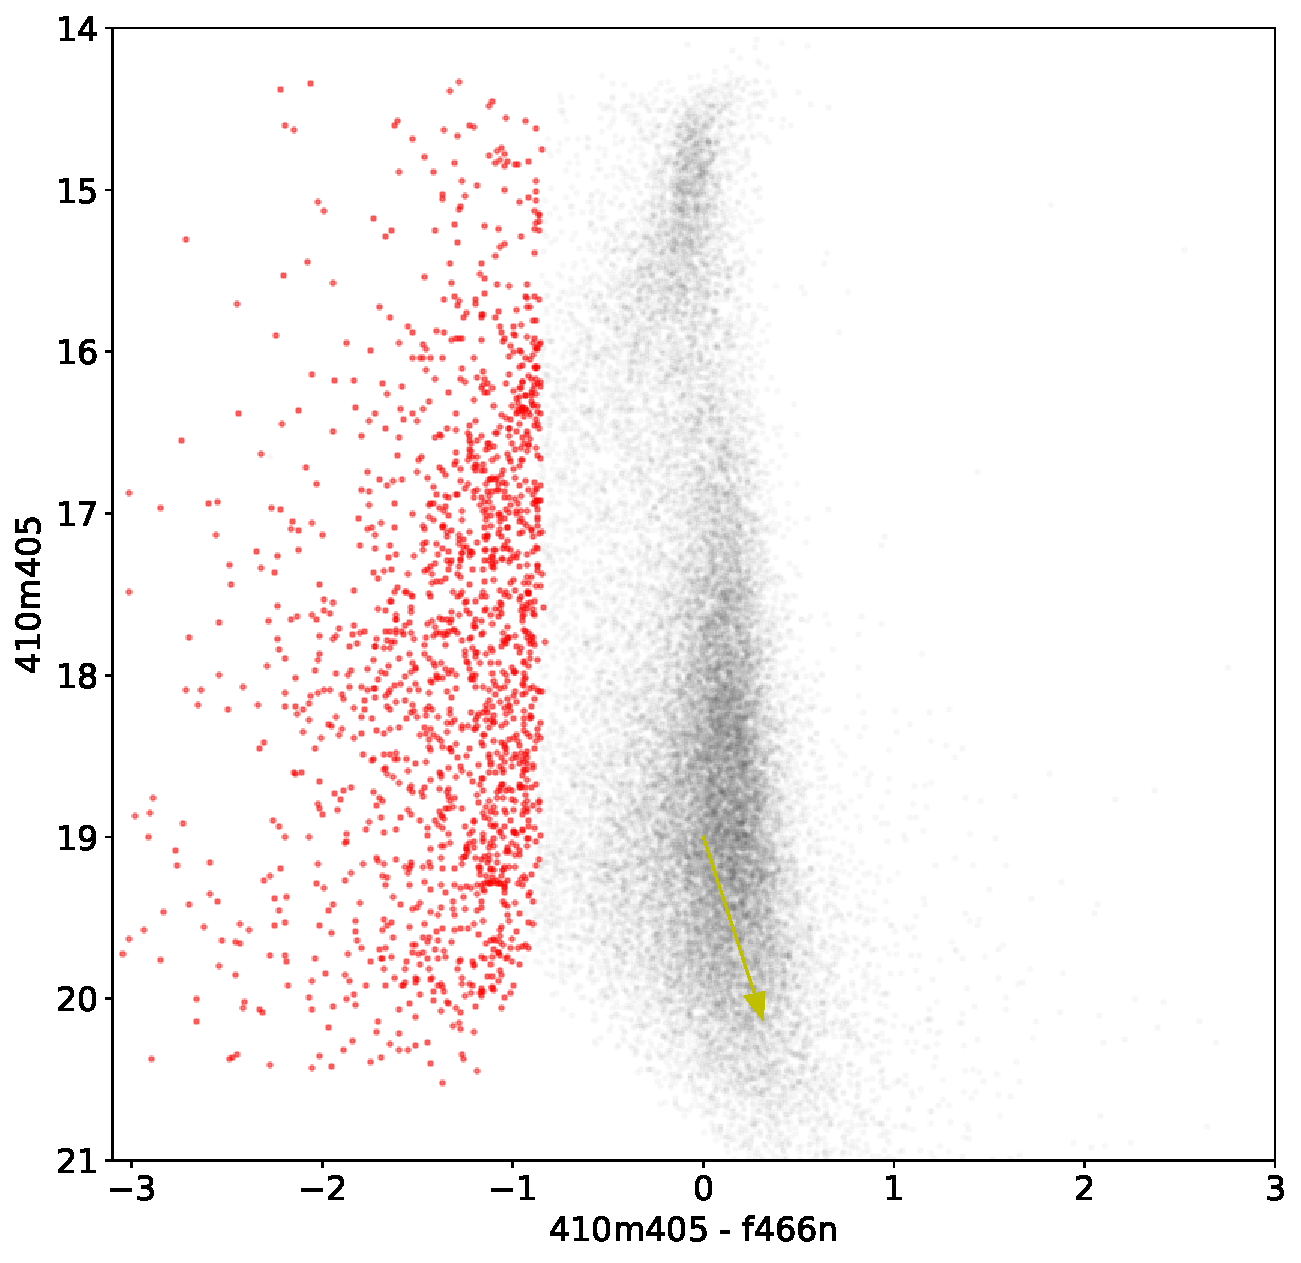
\includegraphics[width=0.49\textwidth]{figures/CMD_F466N_F410MmF405N.pdf}
%     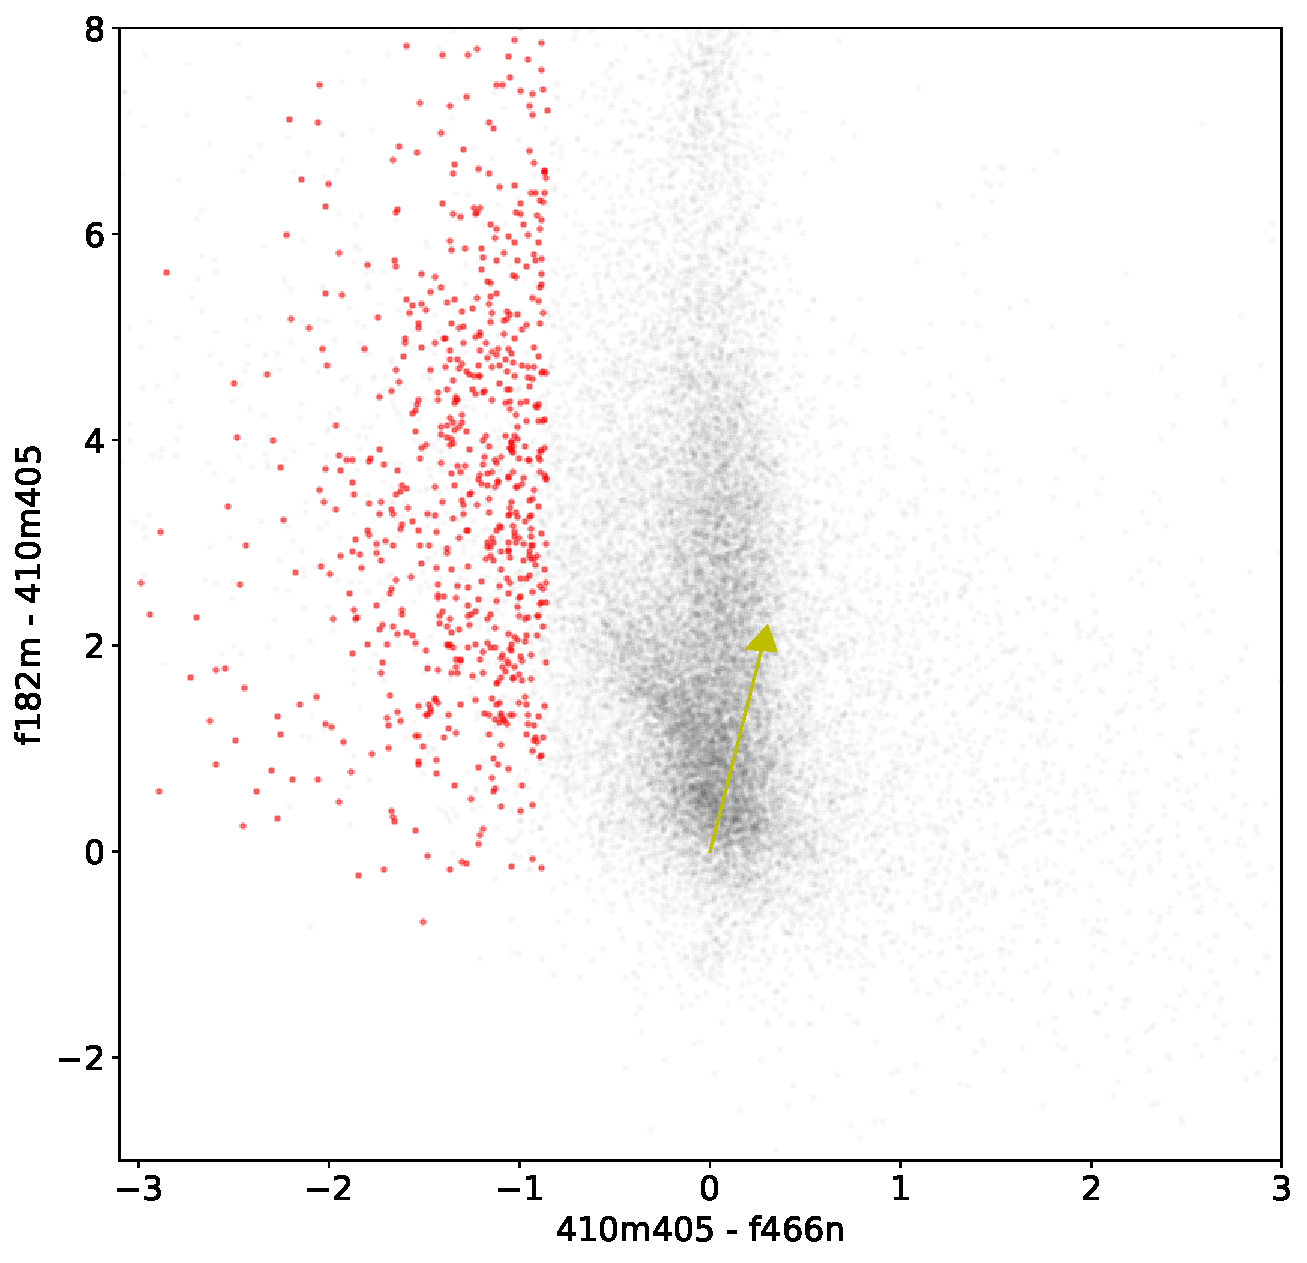
\includegraphics[width=0.49\textwidth]{figures/CCD_ExtinctionVsBlueing.pdf}
%     \caption{
%     (left) Color-magnitude diagram in Br$\alpha$ line-subtracted F410M continuum and the F466N filter.
%     (right) Comparison of the F466N-F410M to F410M-F182M colors.
%     The yellow vector shows the RRP89 reddening vector for $A_V=20$.
%     These stars are shown in Figure \ref{fig:bluestarsextended} and \ref{fig:bluestarsonstars}, though not all stars shown in that figure are present in this one; several stars were identified as blue in F466N-F410M colors but were not detected in F212N.
%     }
%     \label{fig:redvsblue}
% \end{figure}

%\section{CO absorption modeling}


% \subsubsection{Spatial variation of extinction}
% In Figure \ref{fig:extinction_comparison}, the main dark cloud appears much bluer than the surrounding region, however we know this is the region of highest column density and extinction.
% The apparent blue excess is caused by a deficiency of red stars; in this area, the reddening is so great as to render background stars undetectable.
% The `clown vomit' color scheme immediately surrounding the dark cloud indicates that the highest variation in detectable extinction occurs just at the cloud edge, which is expected if stars become undetectable at the highest column densities.

% this section is now covered well earlier
% \subsection{Where are the blue stars?}
% The spatial distribution of the blue stars corresponds with extinction features clearly evident in Figure \ref{fig:bluestarsextended}.
% However, there is also a relative dearth of these stars in the darkest parts of the brick.
% Most likely this is simply a sensitivity issue: stars obscured by too much extinction are not detectable.
% 
% Morphologically, the blue stars appear in locations in the image where there is evidence of extinction from the Brick cloud.
% We therefore expect that the amount of material in front of the star to determine whether a star is significantly blued, and therefore the F466N blueing should be well-correlated with the total dust extinction.
% However, Figure \ref{fig:redvsblue} shows that, at least for the bluest stars, there is no evidence for correlation with extinction.
% This lack of correlation is largely caused by selection bias; to measure extinction with the current data set, we require a detection in the F212N band, so the selected blue sources represent a tiny subset that were detectable in F212N.
% An improved measurement of the correlation with extinction should be possible when future GTO data in additional broad bands become available.